% Created 2013-07-29 Mon 20:04
\documentclass[a4paper,11pt]{article}
\usepackage[utf8]{inputenc}
\usepackage[T1]{fontenc}
\usepackage{hyperref}
\tolerance=1000
\usepackage{fontspec}
\usepackage{biblatex}
\usepackage{graphicx}
\usepackage{fullpage}
\usepackage{caption}
\usepackage{subfig}
\usepackage{hyperref}

\bibliography{report}
\defaultfontfeatures{Mapping=tex-text}
\setromanfont[Ligatures={Common},Numbers={Lining}]{Linux Libertine}

\title{Sokoban: Search in a complex domain}
\author{Yann Chazzalon,  Nicolas Dossou-Gb{\'e}t{\'e}, Tony Chan Ki Hong and Michal Staniaszek}
\date{\today}

\begin{document}

\maketitle

\begin{abstract}
  a brief summary of your project and obtained results
\end{abstract}

\begin{figure}[!ht]
  \captionsetup[subfigure]{labelformat=empty}
  \centering
  \subfloat[\centering Yann Chazallon\\ /01/16]{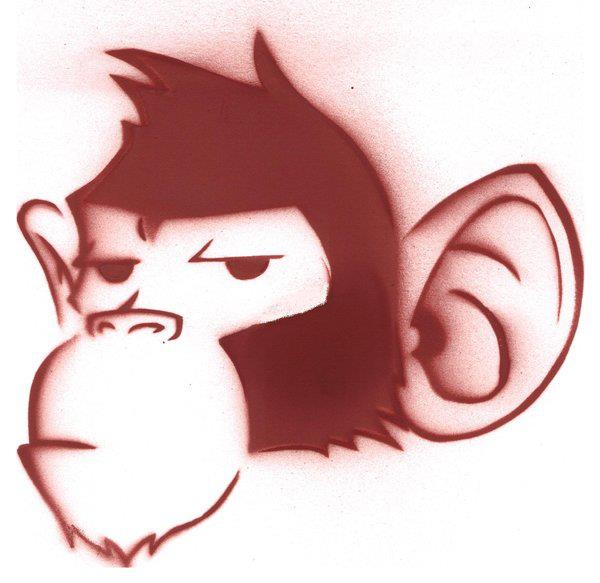
\includegraphics[width=.2\textwidth]{img/yann.jpg}}\quad
  \subfloat[\centering Nicolas Dossou-Gb{\'e}t{\'e}\\ 89/09/26]{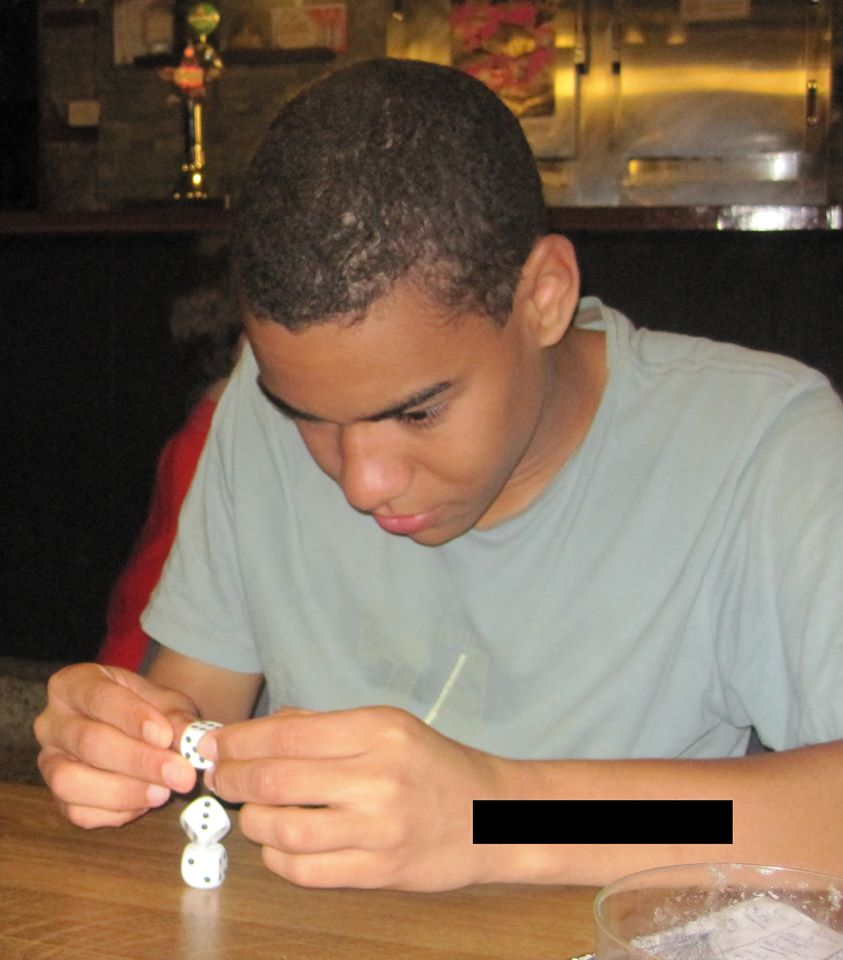
\includegraphics[width=.2\textwidth]{img/nicolas.jpg}}\quad
  \subfloat[\centering Tony Chan Ki Hong\\ /07/25]{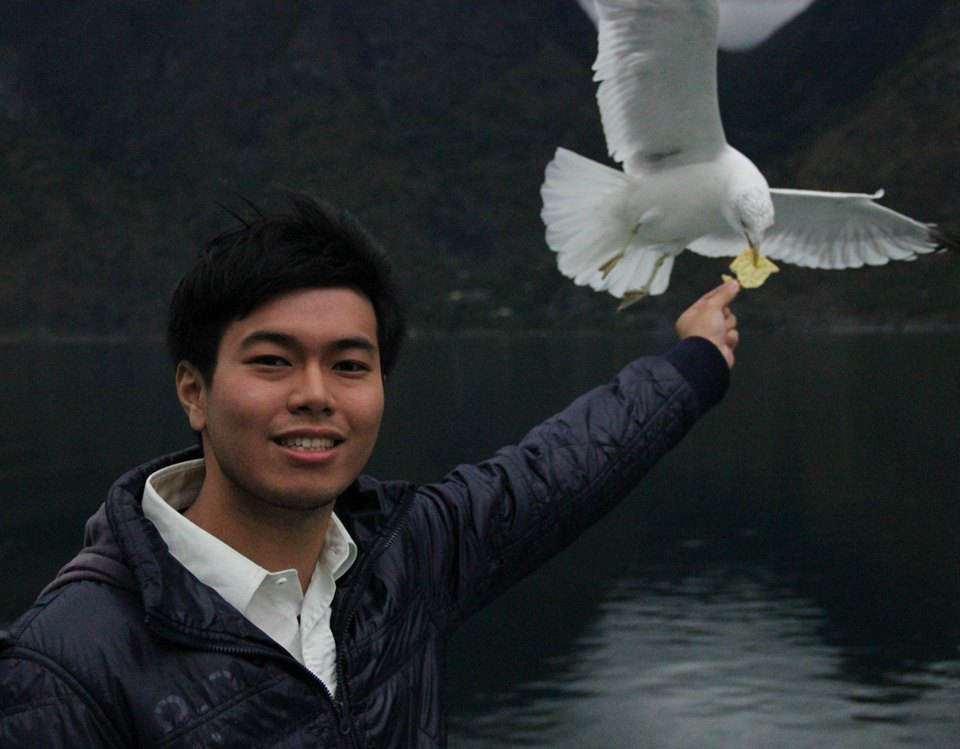
\includegraphics[width=.2\textwidth]{img/tony.jpg}}\quad
  \subfloat[\centering Michal Staniaszek\\ 90/12/07]{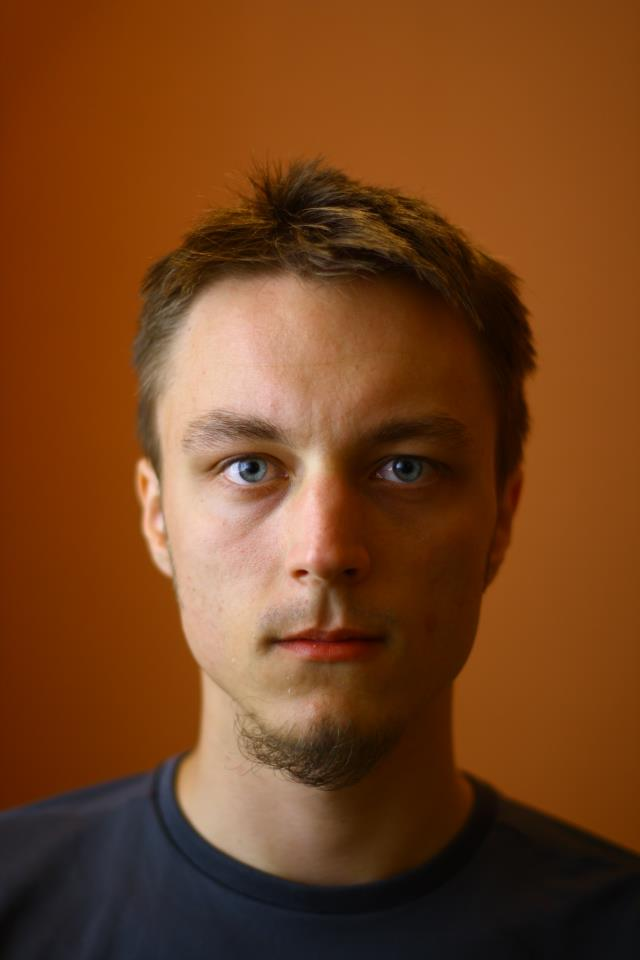
\includegraphics[width=.2\textwidth]{img/michal.jpg}}
\end{figure}

\section{Introduction}
short introduction to the problem and a brief description of how the work was distributed
\section{Method}
a description of your approach to the problem and your method
\section{Implementation}
implementation details (if there are any important ones)
\section{Evaluation}
experimental evaluation and a thorough analysis of your results. This section should include:
How well did your agent do on the different maps?
\section{Discussion}
reflection section dealing with questions: How did you plan to solve the problem? How did you plan the work in the group? What other methods did you try out? What did work/ did not work? Why? How did you end up with the current approach? How did you measure the performance and success during the process? How would you solve it if you were asked to do it again given what you know now?

\printbibliography

\end{document}